\subsection{Estado de fuente y usos}

El estado de fuentes y usos permite examinar los cambios en los activos, pasivos y patrimonio entre dos periodos, facilitando así la evaluación de la eficiencia en el uso de los recursos. Para este proyecto, se mostrará la variación entre el año 1 y el año 2. En la tabla \ref{financiacion} se presenta el estado de fuentes y usos correspondiente a dicho intervalo.

\vspace{2mm}
\begin{minipage}{0.9\textwidth}
\centering
\captionof{table}[{Estado de fuente y usos
}]{ Estado de fuente y usos. }
\label{financiacion}
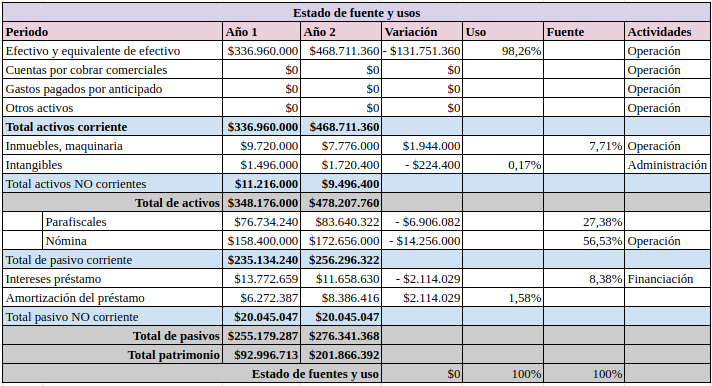
\includegraphics[width=0.9\textwidth]{Content/Images/AF/EstadosDeFuenteYUsos.png}
\footnote{Nota. \textup{Fuente : Autores}}
\end{minipage}

\vspace{2mm}
\begin{minipage}{0.9\textwidth}
\centering
\captionof{table}[{Resumen fuente y usos}]{ Resumen fuente y usos. }
\label{resumen}
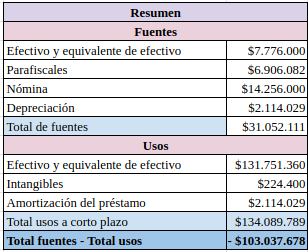
\includegraphics[width=0.9\textwidth]{Content/Images/AF/EstadosDeFuenteYUsosResumen.png}
\footnote{Nota. \textup{Fuente : Autores}}
\end{minipage}
